\documentclass{beamer}

\newenvironment{tightcenter}{%
  \setlength\topsep{0pt}
  \setlength\parskip{0pt}
  \begin{center}
}{%
  \end{center}
}

\mode<presentation>
{
  \usetheme{Copenhagen}
  %%\usecolortheme[RGB={173,222,25}]{structure}
  \usecolortheme[RGB={66,134,244}]{structure}
  \setbeamertemplate{items}[circle]
  \setbeamercovered{transparent}
}

%% zooart binia85

\usepackage[polish]{babel}
\usepackage{chessfss}
\PassOptionsToPackage{hyphens}{url}
\usepackage{hyperref}
\usepackage{qtree}
\usepackage{mathtools}
\usepackage{dirtytalk}
\usepackage{epigraph}
\usepackage{textgreek}
\usepackage[utf8]{inputenc}
\usepackage{times}
\usepackage[T1]{fontenc}
\usepackage{tikz}
\usepackage{csquotes}
\usepackage{amsmath}
\usepackage{fancyvrb}
\usepackage{ulem}
\usepackage{adjustbox}

\newcommand{\prompt}{\phantom{}>\phantom{}>\phantom{}>\ }

\newenvironment{Snippet}{\Verbatim[samepage=true]}{\endVerbatim}

\title{\textbf{The Principles of Functional Programming}}

\author{Panicz Maciej Godek}

\institute{
  \tiny{\href{mailto:godek.maciek@gmail.com}{\textbf{godek.maciek@gmail.com}}} \\
  \normalsize{\url{https://github.com/panicz/writings/tree/master/talks/datamass}}
}

\date{\textbf{datamass.io summit}, 29.09.2017}

\begin{document}

\begin{frame}
  \titlepage
\end{frame}

\begin{frame}{The goals of the talk}
  \begin{itemize} \pause
    \item explain what Functional Programming is \pause
    \item expose some common confusion \pause
    \item debunk some widespread myths \pause
    \item show the value and applicability of FP \pause
    \item and fallacies that arise when \textbf{not using FP}
  \end{itemize}
\end{frame}


\begin{frame}{What is functional programming?} \pause
  Myth \#1: Functional programming isn't well defined. \pause

  \begin{displayquote}
    \textbf{functional programming} -- programming paradigm that
    treats computation as the evaluation of mathematical functions
    and avoids changing-state and mutable data
  \end{displayquote}

  \begin{flushright}
  {\footnotesize \url{https://en.wikipedia.org/wiki/Functional_programming}}
  \end{flushright}
  
\end{frame}

\begin{frame}{Function vs. procedure} \pause
  
  \begin{displayquote}
    \textbf{procedure} -- a sequence of instructions that show
    how to achieve some result, such as to prepare
    or make something
  \end{displayquote}
  \begin{flushright}
    {\footnotesize \url{https://en.wikipedia.org/wiki/Procedure}} \\ \pause
  \end{flushright}
  \ \\
  \texttt{int main(void) \{ \\
    \ \ printf("Hello world!\textbackslash{}n"); \\
    \ \ return 0;\\
    \}}
  
\end{frame}

\begin{frame}{Procedure -- real life example}
  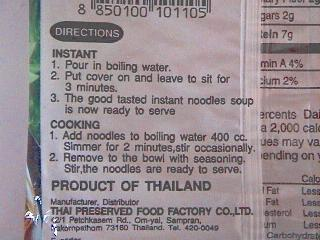
\includegraphics[width=\textwidth]{instant-soup.jpg}
\end{frame}

\begin{frame}{Function (in mathematical sense)}

  \begin{displayquote}
    \textbf{function} -- a relation that associates an input to
    a single output according to some rule
  \end{displayquote}
  \begin{flushright}  
    {\footnotesize \url{https://en.wikipedia.org/wiki/Function}} \\ \pause
  \end{flushright}
  \ \\
  \texttt{int square(int x) \{\\
    \ \ return x * x; \\
    \}} \pause \\
  \ \\
  \begin{center}
    {\footnotesize (a procedure can implement a function)}
  \end{center}
\end{frame}

\begin{frame}{Functions and procedures in standard C library}

  \begin{columns}[T]
    \begin{column}{.48\textwidth}
      \textbf{functions} \\* \pause
      \texttt{tolower} \\* \pause
      \texttt{isdigit} \\* \pause
      \texttt{strlen} \\* \pause
      \texttt{strcmp} \\* \pause
      \texttt{sqrt} \\* \pause
      \texttt{+ - * / < == >} \pause
    \end{column}
    \begin{column}{.48\textwidth}
      \textbf{procedures} \\* \pause
      \texttt{printf} \\* \pause
      \texttt{scanf} \\* \pause
      \texttt{memcpy} \\* \pause
      \texttt{clock} \\* \pause
      \texttt{rand} \\* \pause
      \texttt{++ -\phantom{}- = += *=}
    \end{column}
  \end{columns}
\end{frame}

\begin{frame}{Lambdas} \pause
  Myth \#2: functional programming is about using \textit{lambdas} or
  \textit{closures} or \textit{higher-order functions/procedures}\pause

  \begin{displayquote}
    \textbf{Lambda, Λ, λ} -- is the 11th letter of the Greek alphabet
  \end{displayquote}
  \begin{flushright}
    {\footnotesize \url{https://en.wikipedia.org/wiki/Lambda}} \\ \pause
  \end{flushright}
  \ \\
  \texttt{function make\_counter() \{ \\
    \ \ var counter = 0; \\
    \ \ return function() \{ \\
    \ \ \ \ return ++counter; \\
    \ \ \}; \\
    \}
  }
\end{frame}

\begin{frame}{Parts of speech}
  Myth \#3: objects are like nouns and functions are like verbs \\ \pause
  \ \\
  \texttt{insertions:: a -> [a] -> [[a]]\\ \pause
    insertions x []\ \ \ \ = [[x]] \\
    insertions x (h:t) = [(x:h:t)] ++ entwined\\
    \ \ where entwined = (map\,(h:)\,(insertions~x~t))
  } \\ \pause
  \ \\
  \texttt{e.g.\,insertions 0 [1,2,3] ===>\\
    \ \ [[0,1,2,3],[1,0,2,3],[1,2,0,3],[1,2,3,0]]
  } \\ \pause
  \ \\
  other examples: \texttt{powerset}, \texttt{permutations},
  \texttt{sorted}
  
\end{frame}

\begin{frame}{Imperative functional programming} \pause
  Myth \#4: (pure) functions cannot be implemented in non-functional
  (imperative) way \\ \pause
  \ \\
  \begin{columns}[T] % align columns
    \begin{column}{.48\textwidth}
      %\rule{\linewidth}{4pt}
      \begin{small}
        \texttt{int factorial(int n) \{\\*
          \ \ int result = 1;\\*
          \ \ while (n > 0)\\*
          \ \ \ \ result *= n-\phantom{}-;\\*
          \ \ return result;\\*
          \}}
      \end{small}
    \end{column}%
    \hfill%
    \pause
    \begin{column}{.48\textwidth}
      \begin{small}
        \texttt{int factorial(int n) \{\\*
          \ \ if (n < 1) return 1; \\*
          \ \ else return\\*
          \ \ \ \ n*factorial(n-1);\\*
          \}}
      \end{small}
    \end{column}
  \end{columns} 
\end{frame}

\begin{frame}{Why functional programming?} \pause
  Myth \#5: you need to understand Category Theory to use
  functional programming \\ \pause
  \ \\ \pause
  {\large Imperative programs explain how to \textbf{do} things
  (perform \textit{actions}), while
  functional programs \textbf{mean} things (refer to \textit{objects}).}
  
\end{frame}

\begin{frame}{Sum of squares of initial 7 prime numbers (procedural)} \pause
  \texttt{counter := 7\\* \pause
number := 0\\* \pause
sum := 0\\* \pause
while(counter > 0):\\* \pause
\ \ \ \ if is\_prime(number):\\* \pause
\ \ \ \ \ \ \ \ sum := sum + number\^{}2\\* \pause
\ \ \ \ \ \ \ \ counter := counter - 1\\* \pause
\ \ \ \ counter := counter + 1\\* 
  } \ \\ \pause
  After its execution, the \texttt{sum} variable contains the
  desired value
\end{frame}

\begin{frame}{Sum of squares of initial 7 prime numbers (functional)} \pause
  \texttt{(sum (map square \\
    \ \ \ \ \ \ \ \ \ \ (initial 7 (only prime?\,\,numbers))))} \\ \ \\ \pause
  \begin{center}
    {\footnotesize (no need to tell where to look for the result)}
  \end{center}
\end{frame}

\begin{frame}{Sum of squares of initial 7 prime numbers (definitions)} \pause
  \texttt{(define (numbers-from first)\\
    \ \ `(,first .\,\,,(numbers-from (+ first 1))))\\
    \ \\ \pause
    (define numbers (numbers-from 0))\\
    \ \\ \pause
    (define (only qualifying?\,\,elements)\\ \pause
    \ \ (match elements\\ \pause
    \ \ \ \ ('()\\
    \ \ \ \ \ '())\\ \pause
    \ \ \ \ (`(,first .\,\,,rest)\\ \pause
    \ \ \ \ \ (if (qualifying?\,\,first)\\
    \ \ \ \ \ \ \ \ \ `(,first .\,\,,(only qualifying?\,\,rest))\\ \pause
    \ \ \ \ \ \ \ (only qualifying?\,\,rest)))))\\
    }    
\end{frame}

\begin{frame}{Sum of squares of initial 7 prime numbers (definitions)} \pause
  \texttt{(define (initial n elements)\\ \pause
    \ \ (if (= n 0)\\
    \ \ \ \ \ \ '()\\ \pause
    \ \ \ \ (let ((`(,first .\,\,,rest) elements))\\
    \ \ \ \ \ \ \ `(,first .\,\,,(initial (- n 1) rest)))))\\
    \ \\ \pause
    (define (sum numbers)\\ \pause
    \ \ (match numbers\\ \pause
    \ \ \ \ ('()\\
    \ \ \ \ \ 0)\\ \pause
    \ \ \ \ (`(,number .\,\,,other-numbers)\\
    \ \ \ \ \ (+ number (sum other-numbers)))))
  }
\end{frame}

\begin{frame}{The substitution model of computation}
  \texttt{(sum \\
    \ \ (map square \\
    \ \ \ \ \ (initial 7\\
    \ \ \ \ \ \ \ \ (only prime?\,\,\textbf{numbers}))))}
\end{frame}

\begin{frame}{The substitution model of computation}
  \texttt{(sum \\
    \ \ (map square \\
    \ \ \ \ \ (initial 7\\
    \ \ \ \ \ \ \ \ (only prime?\,\,\textbf{'(0 1 2 3 4 5 6 ...)}))))}
\end{frame}

\begin{frame}{The substitution model of computation}
  \texttt{(sum \\
    \ \ (map square \\
    \ \ \ \ \ (initial 7\\
    \ \ \ \ \ \ \ \ \textbf{(only prime?\,\,'(0 1 2 3 4 5 6 ...))})))}
\end{frame}

\begin{frame}{The substitution model of computation}
  \texttt{(sum \\
    \ \ (map square \\
    \ \ \ \ \ (initial 7\\
    \ \ \ \ \ \ \ \ \textbf{'(2 3 5 7 11 13 19 23 29 31 37 ...)})))}
\end{frame}


\begin{frame}{The substitution model of computation}
  \texttt{(sum \\
    \ \ (map square \\
    \ \ \ \ \ \textbf{(initial 7\\
    \ \ \ \ \ \ \ \ '(2 3 5 7 11 13 19 23 29 31 37 ...))}))}
\end{frame}

\begin{frame}{The substitution model of computation}
  \texttt{(sum \\
    \ \ (map square \\
    \ \ \ \ \ \textbf{'(2 3 5 7 11 13 19)}))\\
    \ }
\end{frame}

\begin{frame}{The substitution model of computation}
  \texttt{(sum \\
    \ \ \textbf{(map square \\
    \ \ \ \ \ '(2 3 5 7 11 13 19))})\\
    \ }
\end{frame}

\begin{frame}{The substitution model of computation}
  \texttt{(sum \\
    \ \ \textbf{'(4 9 25 49 121 169 361)})\\
    \ \\
    \ }
\end{frame}

\begin{frame}{The substitution model of computation}
  \texttt{\textbf{(sum \\
    \ \ '(4 9 25 49 121 169 361))}\\
    \ \\
    \ }
\end{frame}

\begin{frame}{Binding vs. assignment} \pause
  Myth \#6: binding and assignment are the same thing \\ \pause
  \begin{itemize}
  \item \textbf{definition} -- creates a new binding in the
    current scope \\ \pause
    \texttt{(define variable value)}\pause
  \item \textbf{assignment} -- changes the value bound by
    a variable in the current scope \\ \pause
    \texttt{(set!\,\,variable new-value)}
  \item \textbf{binding} -- creates a new scope,
    possibly shadowing some existing binding \\ \pause
    \texttt{(let ((variable some-value)) \\
      \ \ {\scriptsize ;; any outer binding of `variable` is shadowed here} \\
      \ \ ...) \\ \pause
      {\scriptsize ;; outer context -- 'variable' has its original value}
      }
  \end{itemize}
\end{frame}

\begin{frame}{Immutability} \pause
  {\large \textbf{How can you change the meaning of a word?}} \pause
  \ \\
  \begin{itemize}
  \item by explaining the new meaning to everyone \pause
  \item by modifying the structure of the brains of all the people \pause
  \end{itemize}
  {\footnotesize What about the previous usages of that word?}
\end{frame}

\begin{frame}{Other examples of immutable systems} \pause
  \begin{itemize}
    \item functional package managers (NIX, Guix) \pause
    \item Git \pause
    \item history (can't be undone)
  \end{itemize}
\end{frame}

\begin{frame}{Problems with mutation} 
  Is \texttt{x += y} a shorthand for \texttt{x = x + y}? \\ \pause
  \ \\
  Let's see... \\ \pause
  \begin{columns}[T] % align columns
    \begin{column}{.48\textwidth}
      %\rule{\linewidth}{4pt}
      \begin{small}
        \texttt{\prompt{} x = 5\\ \pause
          \prompt{} x = x + 3 \\ \pause
          \prompt{} x \\ \pause
          8 \\ \pause
          \ \\ \ \\ \ \\ \ \\ \ \\ \ \\ \ \\ \ \\
        }
      \end{small}
    \end{column}%
    \hfill%
    \begin{column}{.48\textwidth}
      \begin{small}
        \texttt{\prompt{} x = 5\\ \pause
          \prompt{} x += 3 \\ \pause
          \prompt{} x \\ \pause
          8 \\
          \ \\ \ \\ \ \\ \ \\ \ \\ \ \\ \ \\ \ \\
        }
      \end{small}
    \end{column}
  \end{columns} 
\end{frame}

\begin{frame}{Problems with mutation} 
  Is \texttt{x += y} a shorthand for \texttt{x = x + y}? \\
  \ \\
  Interference test \\ \pause
  \begin{columns}[T] % align columns
    \begin{column}{.48\textwidth}
      %\rule{\linewidth}{4pt}
      \begin{small}
        \texttt{\prompt{} x = 5\\ \pause
          \prompt{} y = x\\ \pause
          \prompt{} x = x + 3 \\ \pause
          \prompt{} x \\ \pause
          8\\ \pause
          \prompt{} y \\ \pause
          5 \\
          \ \\
          \ \\
          \ \pause
        }
      \end{small}
    \end{column}%
    \hfill%
    \begin{column}{.48\textwidth}
      \begin{small}
        \texttt{\prompt{} x = 5\\ \pause
          \prompt{} y = x\\ \pause
          \prompt{} x += 3 \\ \pause
          \prompt{} x \\ \pause
          8\\ \pause
          \prompt{} y\\ \pause
          5 \\
          \ \\
          \ \\
          \ 
        }
      \end{small}
    \end{column}
  \end{columns} 
\end{frame}


\begin{frame}{Spooky action at a distance}
  Is \texttt{x += y} a shorthand for \texttt{x = x + y}? \\
  \ \\
  Sanity check \\ \pause
  \begin{columns}[T] % align columns
    \begin{column}{.48\textwidth}
      %\rule{\linewidth}{4pt}
      \begin{small}
        \texttt{\prompt{} x = [1, 2, 3] \\ \pause
          \prompt{} y = x\\ \pause
          \prompt{} x = x + [4, 5] \\ \pause
          \prompt{} x \\ \pause
          \phantom{} [1, 2, 3, 4, 5] \\ \pause
          \prompt{} y \\ \pause
          \phantom{} [1, 2, 3] \pause
        }
      \end{small}
    \end{column}%
    \hfill%
    \begin{column}{.48\textwidth}
      \begin{small}
        \texttt{\prompt{} x = [1, 2, 3] \\ \pause
          \prompt{} y = x\\ \pause
          \prompt{} x += [4, 5] \\ \pause
          \prompt{} x \\ \pause
          \phantom{} [1, 2, 3, 4, 5] \\ \pause
          \prompt{} y\\ \pause
          \phantom{} [1, 2, 3, 4, 5] \pause \# oops!
        }
      \end{small}
    \end{column}
  \end{columns} 
\end{frame}

\begin{frame}{Problems with mutability}
  \begin{small}
    \texttt{\prompt def f(x=\{\}):\\
      ... \ \ \ \ return x\\ \pause
      \prompt x = f()\\ \pause
      \prompt x \\ \pause
      \{\} \\ \pause
      \prompt x['a'] = 5 \\ \pause
      \prompt x \\ \pause
      \{'a': 5\} \\ \pause
      \prompt y = f()\\ \pause
      \prompt y\\ \pause
      \{'a': 5\} \pause \# oops!
    }
  \end{small}
\end{frame}


\begin{frame}{Pros and cons} \pause
  \textbf{Advantages:} \pause
  \begin{itemize}
  \item code is easier to read and refactor and less prone to errors \pause
  \item no control flow means more flexible interpretation \pause
  \item better multicore optimization \pause
  \item we don't care what the computer do will \pause
  \end{itemize}

  \textbf{Disadvantages:} \pause
  \begin{itemize}
  \item may cause performance penalties \pause
  \item difficult to reason about resource usage \pause
  \item often leads smug programmers to awkward abstractions \pause
  \item we don't know what the computer will do
  \end{itemize}
\end{frame}


\end{document}
